\documentclass[12pt,3p]{elsarticle}
\usepackage{tikz}
\usetikzlibrary{positioning,chains,fit,shapes,calc}
\newcommand{\swastik}[1]{%
    \begin{tikzpicture}[#1]
        \draw (-1,1)  -- (-1,0) -- (1,0) -- (1,-1);
        \draw (-1,-1) -- (0,-1) -- (0,1) -- (1,1);
    \end{tikzpicture}%
}

\tikzset{
    treenode/.style={align=center, inner sep=0pt},
    % Receiver Node
    node_rec/.style = {treenode, circle, white, font=\bfseries, draw=black, fill=black, text width=0.8cm},
    % Sender Node
    node_sen/.style = {treenode, circle, red, draw=red, very thick, text width=0.8cm}
}
\usepackage{graphicx}
\usepackage{amssymb}

\makeatletter
\def\ps@pprintTitle{%
 \let\@oddhead\@empty
 \let\@evenhead\@empty
 \def\@oddfoot{}%
 \let\@evenfoot\@oddfoot}
\makeatother
\begin{document}

\begin{frontmatter}

\title{\swastik{scale=0.2} Solution to problem 9 in Assignment 1 \swastik{scale=0.2}}

\author{Sourabh Aggarwal}
\address{111601025@smail.iitpkd.ac.in}

\end{frontmatter}
\section{Problem Desc}
\label{sec1}
Let $G = (V, E)$ be a graph with nonnegative edge costs. $S$, the $senders$
and $R$, the $receivers$, are disjoint subsets of $V$ . The problem is to find a
minimum cost subgraph of $G$ that has a path connecting each receiver to a sender (any sender suffices). Partition the instances into two cases: $S \cup R = V$
and $S \cup R \neq V$ . Show that these two cases are in P and NP-hard, respectively.
For the second case, give a factor 2 approximation algorithm.
\textbf{Hint}: Add a new vertex which is connected to each sender by a zero cost
edge. Consider the new vertex and all receivers as required and the remaining
vertices as Steiner, and find a minimum cost Steiner tree.

\section{Soln for first case}
We would first need a couple of observations. I will denote $r_i$ as a vertex in $R$ and $s_i$ as a vertex in $S$.

\textbf{Observation 1: }Optimum soln would consist of union of subtrees. That is, optimum soln need not be a subtree (as consider figure 1) and obviously optimum soln need not contain cycle as even if optimum soln contains a cycle where one of the cycle's edge has weight 0, then we can safely disregard this edge (so from now on, I will assume that optimum soln doesn't contain cycles).
\begin{figure}[!h]
    \centering
    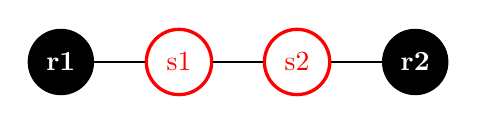
\begin{tikzpicture}[level/.style = {sibling distance=2cm, level distance=1.5cm}]

        \node[node_rec]{r1}
            child[grow=right]{node[node_sen]{s1}
                child[grow=right]{node[node_sen]{s2}
                    child[grow=right]{node[node_rec]{r2}}}
            };
    \end{tikzpicture}
    \caption{In an optimal soln of this graph, edge (s1, s2) will not be present irrespective of weight}
\end{figure}


\textbf{Observation 2: }For a particular reciever, the nearest vertex in $S$ in optimal soln need not be the most nearest vertex of $S$. See figure 2.

\begin{figure}[!h]
    \centering
    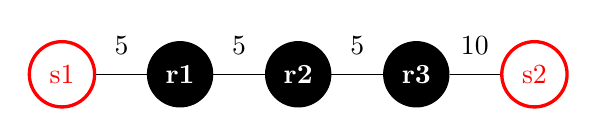
\begin{tikzpicture}[level/.style = {sibling distance=2cm, level distance=1.5cm}]

        \node[node_sen]{s1}
            child[grow=right]{node[node_rec]{r1} 
                child[grow=right]{node[node_rec]{r2}
                    child[grow=right]{node[node_rec]{r3}
                        child[grow=right]{node[node_sen]{s2}
                        edge from parent node[label=10]{}}
                    edge from parent node[label=5]{}}
                edge from parent node[label=5]{}}
            edge from parent node[label=5]{}
            };
    \end{tikzpicture}
    \caption{Here optimal soln has all edges except (r3, s2) even though s2 is nearer than s1 to r3}
\end{figure}

\textbf{Observation 3: }From first observation it follows that the optimum soln would consist of union of many subtrees and observe that each of these subtrees should contain exactly one vertex from $S$. 

\textit{Proof: }Suppose there existed more than one vertex from $S$ in a particular subtree $T_1$. Consider any two nearest vertices $s_1, s_2, (s_1 \neq s_2)$ in $S \cap T_1$. Path from $s_1$ to $s_2$ in $T_1$ would look like $s_1, (r_k)^*, s_2$ where $(r_k)^*$ denotes a possible sequence (could be empty) of vertices in $R$. If $(r_k)^*$ is empty then delete edge $(s_1, s_2)$ and if it is not empty, i.e., sequence is of the form $s_1, r_{k_1}, ..., s_2$ then delete edge $(s_1, r_{k_1})$. \textit{Note: We could safely delete as deleting doesn't increase cost and is also maintaining connectivity}. Continuing this way, we have proved the observation.

From all these observation it follows that if we add an auxiliary vertex $aux$ and add the edges $(s_i, aux), \forall s_i \in V$ with cost 0 (let the set of our new created edges be $E_{aux}$ then the new set of edges, $E_{new} = E \cup E_{aux}$), the problem reduces to finding the minimum cost spanning tree provided we have already added $E_{aux}$ to our minimum cost spanning tree. \textit{Note: After recieving MST, revmove $E_{aux}$ from it to get the actual soln}.

\textit{Proof: }As our MST would already contain all edges of $E_{aux}$, \textit{Observation 3} is satisfied as, if after removing $E_{aux}$ from MST we get a particular subtree with more than one vertex in $S$ then cleary by adding $E_{aux}$ we would get a cycle, thus our subtree will not contain more than one vertex in $S$ and obviously since we are finding MST on this new graph, it will be connected, thus each vertex in $R$ will be connected to some vertex in $S$. And by the property of MST we have recieved the minimum cost soln. (Note: In case $R \cup S \neq V$ then this soln would fail as it will force to find MST where each vertex even other than $R$ and $S$ is connected, which clearly isn't required in problem constraint. Also note that, since edges can have zero weight, there could be an edge between two vertices of $S$ with zero weight thus it is required for us to add $E_{aux}$ initially to our MST as algorithms (say \textit{Kruskal}) may try to add that original edge first to the forest.)

\section{Soln for second case}
Clearly, observation 1, 2, 3, from previous case still holds. Now we will again add $E_{aux}$ to $E$ giving $E_{new} = E \cup E_{aux}$. Now due to similar reasons instead of finding Minimum Cost Spanning Tree, the problem reduces to finding Minimum Cost Steiner Tree where the set of required vertices is $R \cup aux$ of which we already have a 2 factor approximation algorithm (done in class). 

But to prove that soln under this case is NP Hard we can reduce the Minimum Cost Steiner Tree problem to our problem as follows:

Let the set of required vertices be denoted by $M$. Choose any one vertex of $M$ and put it to set $S$ and put the remaining vertices to $R$. Now if we get soln for this instance, that soln would exactly be the Minimum Cost Steiner Tree (as all the vertices of $R$ will be connected to that single vertex in $S$, thus all the vertices of $R$ are in turn connected with each other). Thus our problem is NP Hard.
\end{document}
